\appendix
\pagenumbering{Roman}


\newappendix{Obsah elektronické přílohy}
Zdrojové kódy firmware, software, návrh hardwarového řešení, elektronické
simulace, jakož i zdrojový kód této práce využívající systému pro počítačovou
sazbu \LaTeX{} jsou k práci přiloženy jako elektronická příloha. Ta je rozdělena
do několika adresářů:
\dirtree{%
    .1 /.
    .2 figures/\DTcomment{obrázky použité v práci}.
    .2 prilohy/\DTcomment{elektronické přílohy}.
    .2 script/\DTcomment{skripty a jendoduché programy používané při zpracovávání práce}.
    .2 sim/\DTcomment{simulace elektronických obvodů}.
    .3 models/\DTcomment{dodatečné SPICE modely součástek}.
    .3 *.asc\DTcomment{LTspice simulace}.
    .3 *.txt\DTcomment{data exportovaná z LTspice simulací}.
    .3 graf-common.gpi\DTcomment{společná nastavení pro všechny grafy ze simulací}.
    .3 graf-*.gpi\DTcomment{zdrojové kódy \shellcmd{gnuplot} grafů ze simulací}.
    .2 *.tex\DTcomment{\LaTeX{} zdrojové kódy práce}.
    .2 Makefile\DTcomment{nastavení build systemu GNU make}.
    .2 reference.bib\DTcomment{informace o použité literatuře}.
    .2 tests\DTcomment{skript kontrolující kvalitu práce, spouštěný build systémem}.
}
\todo[inline]{obsah elektronicke prilohy -- vsechny git repo, ...}



\clearpage
\newappendix{Získávání snímků obrazovky z~digitálního osciloskopu Agilent~54621A}
Autorův digitální osciloskop Agilent~54621A má poškozenou disketovou mechaniku,
proto není možné využít standardní metody získávání snímků obrazovky
a~textových dat. Přenos dat přes disketu funguje, ale je velmi nespolehlivý
a~často vede k jejich ztrátě. Pro účely tvorby dokumentace pro tuto práci byl
vyvinut jednoduchý počítačový program umožňující čtení obrázků ve formátu BMP
přes sériový port RS-232.

Je potřeba použít RS-232 kabel zapojený podle diagramu v dokumentaci
osciloskopu.

\begin{figure}[htbp]
    \centering
    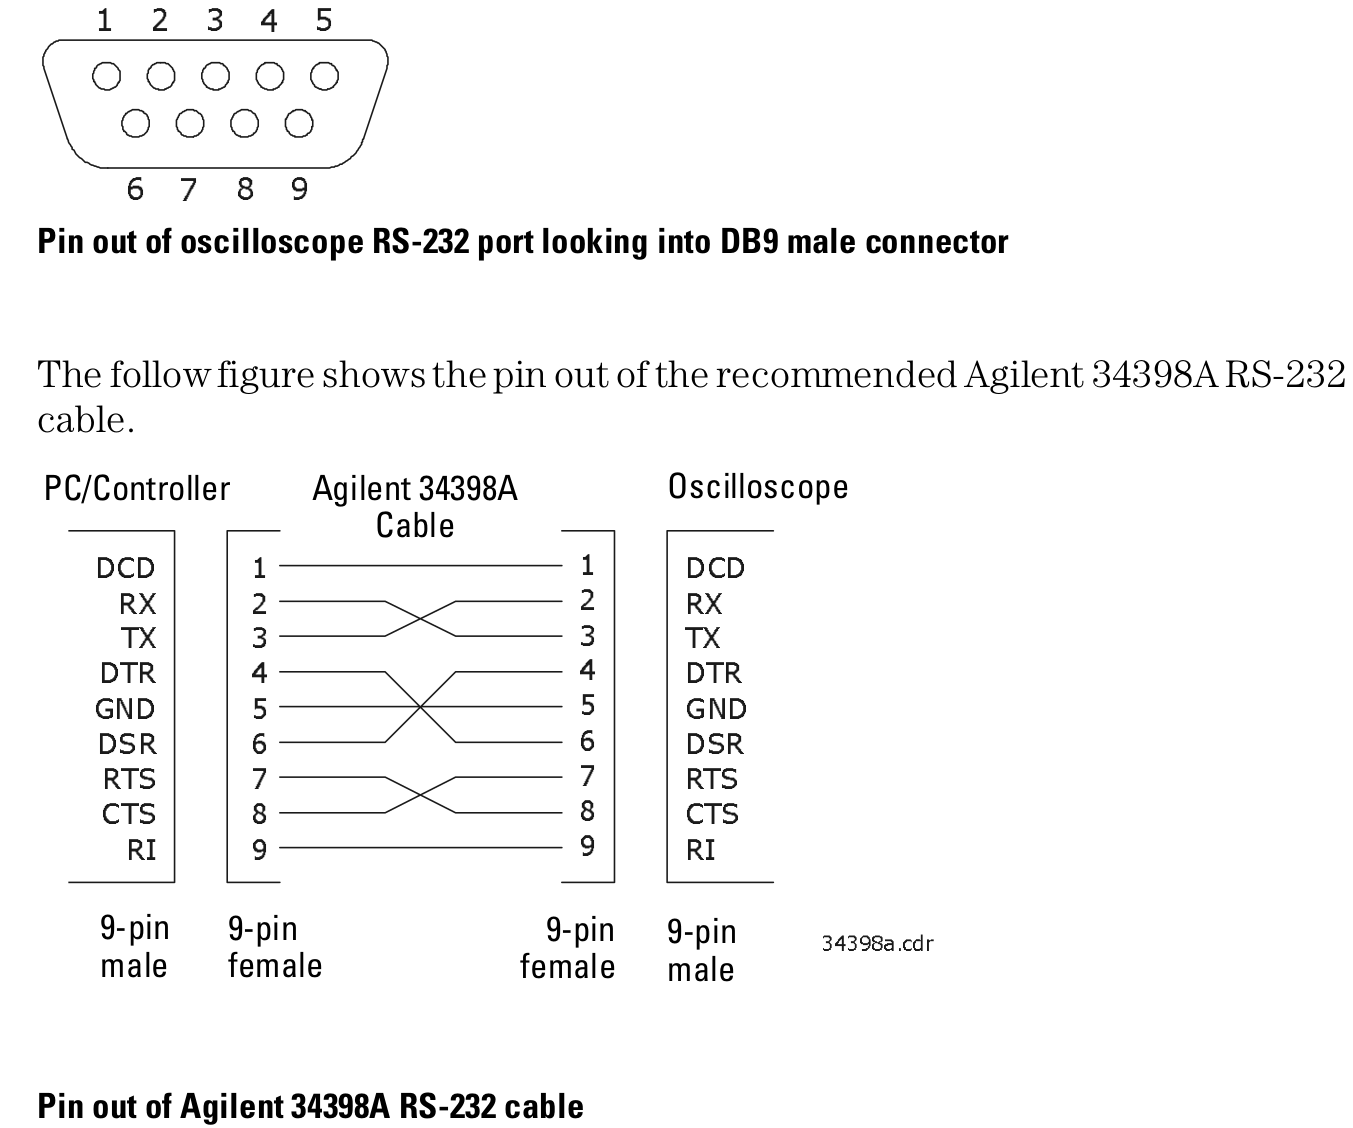
\includegraphics[width=\textwidth]{Agilent-RS232-pinout}
    \caption{%
        Zapojení kabelu pro propojení osciloskopu Agilent~54621A
        s~počítačem~\cite{Agilent54621Auser}
    }
    \label{fig:agilent RS232 pinout}
\end{figure}

Program napsaný v jazyce Python je uložen v souboru \filename{scrot}:
\lstinputlisting[language=Python,style=numbers]{prilohy/scrot}

Po získání nekomprimovaného obrázku ve formátu BMP je vhodné provést
bezztrátovou konverzi do formátu PNG příkazem \shellcmd{convert} z balíčku
\texttt{imagemagick}.
Příklad použití v prostředí operačního systému GNU/Linux:
\begin{lstlisting}[style=terminal]
$ ./scrot -h
usage: scrot [-h] device file

positional arguments:
  device      Serial port the scope is attached to
  file        File to write the output to

optional arguments:
  -h, --help  show this help message and exit

$ ./scrot /dev/ttyUSB1 nazev-souboru
Screen image written to nazev-souboru.bmp
$ convert nazev-souboru.bmp nazev-souboru.png
$
\end{lstlisting}


\todo[inline]{%
    dalsi prilohy
}



\clearpage
\newappendix{Koncový zesilovač s TDA2030}
\label{app:TDA2030}
Při testování zvukového výstupu byl použit jednoduchý nízkofrekvenční koncový
zesilovač s integrovaným obvodem TDA2030, který autor této práce sestavil
v roce 2016 v rámci soutěže v radiotechnice. Na následujícím obrázku je
zobrazen osazovací plán jeho desky plošných spojů a seznam součástek. Schéma
zapojení bohužel není dostupné.
V souboru \filename{prilohy/TDA2030-dokumentace.pdf} je vše, co se zachovalo
z dokumentace tohoto výrobku. Autorem návrhu je Petr Vild OK7PV.

\noindent
\includegraphics[page=2, clip, bb=20mm 89mm 175mm 270mm, width=1.0\textwidth]{prilohy/TDA2030-dokumentace.pdf}
